\documentclass[11pt]{article}
\usepackage[margin=1in]{geometry}
\usepackage[T1]{fontenc}
\usepackage[utf8]{inputenc}
\usepackage{lmodern}
\usepackage{microtype}
\usepackage{amsmath,amssymb,amsthm,mathtools}
\usepackage{booktabs}
\usepackage{array}
\usepackage{enumitem}
\usepackage{graphicx}
\usepackage{tikz}
\usetikzlibrary{arrows.meta,positioning}
\usepackage{natbib}
\usepackage{xurl}
\usepackage[hidelinks]{hyperref}
\usepackage{orcidlink}

\title{SecureParseNet: Differentiable Perceptual Hashing for Integrity-Aware Semantic Segmentation}
\author{Aryan Singh Chandel\,\orcidlink{0009-0007-1774-2480}\\
RJIT (Rustamji Institute of Technology), Gwalior, India\\
\texttt{aryansingh19gh@gmail.com}}
\date{June 26, 2026}

\newtheorem{definition}{Definition}
\newtheorem{assumption}{Assumption}
\newtheorem{proposition}{Proposition}
\raggedbottom
\emergencystretch=2em

\begin{document}
\maketitle

\begin{abstract}
Lightweight segmentation systems are attractive for deployment on edge devices, but their small parameter budgets often leave them highly vulnerable to adversarial perturbations. SecureParseNet addresses this problem by coupling a MobileNetV3-style segmentation backbone with a differentiable perceptual-hash head that monitors structural integrity in the output space. This manuscript rebuilds the supplied PDF into a more formal research paper: it specifies the differentiable hash operator, clarifies the multi-objective training logic, states measurable claims for tamper detection and segmentation robustness, and packages the existing convergence, attack, and confusion-matrix results into a cleaner methodology-oriented narrative. The core idea is that a segmentation network can be made more deployment-safe when integrity verification is treated as a first-class differentiable objective rather than as a post hoc alarm.
\end{abstract}

\section{Introduction}
Semantic segmentation is a dense decision problem, so even small perturbations can alter many output pixels at once. On safety-critical edge platforms, that fragility is harder to tolerate because the systems are often lightweight, latency-constrained, and exposed to uncontrolled environments. Backbone compression improves efficiency, but it does not by itself protect the model from adversarial or tampering-style disturbances \citep{howard2019mobilenetv3,goodfellow2015explaining}.

The motivating idea of SecureParseNet is simple: if the segmentation output is structurally corrupted, the system should not only degrade gracefully but also know that it has been compromised. We therefore pair a segmentation decoder with an integrity head that computes a differentiable perceptual signature over low-frequency output structure, adapting the perceptual-hash tradition to an end-to-end trainable setting \citep{zauner2010implementation}. The paper's claim is not that integrity hashing alone solves adversarial robustness. The sharper claim is that a differentiable integrity objective can provide a reliable detection signal even when semantic quality begins to degrade.

\paragraph{Contributions.}
\begin{enumerate}[leftmargin=*]
\item We formalize a differentiable perceptual hashing layer built from low-frequency transform coefficients and soft thresholding.
\item We define segmentation, integrity, and attack-detection estimands separately rather than collapsing them into a single robustness score.
\item We restate the reported FGSM results as explicit measurement claims about IoU degradation and integrity deviation.
\item We scaffold the supplied figures and table into a fuller manuscript structure for later empirical expansion.
\end{enumerate}

\section{Formal Setup}
Let $X\in[0,1]^{H\times W\times C}$ be an input image, let $E$ and $D$ denote encoder and decoder, and let $Y_{\mathrm{seg}}=D(E(X))$ be the segmentation probability map.

\begin{definition}[Low-frequency coefficient block]
Let $F\in\mathbb{R}^{H\times H}$ and $G\in\mathbb{R}^{W\times W}$ denote orthonormal transform matrices, and let $P_k$ extract the leading $k\times k$ block. For a single-channel segmentation score map $Y$, define
\[
L(Y)=P_k FYG^\top P_k^\top.
\]
In the current manuscript, $F$ and $G$ are taken as DCT bases and $k=8$.
\end{definition}

\begin{definition}[Differentiable perceptual hash]
Let $L(Y_{\mathrm{seg}})$ denote a selected block of low-frequency coefficients from a 2D spectral transform of the segmentation output. The differentiable perceptual hash is
\[
H_{\mathrm{soft}}(X)=\frac{1}{2}\left(1+\tanh\bigl(\beta(L(Y_{\mathrm{seg}})-\mu_L)\bigr)\right),
\]
where $\mu_L$ is the mean of the selected coefficients and $\beta>0$ is a temperature parameter.
\end{definition}

\begin{definition}[Integrity deviation]
Given a clean reference signature $h^\star$ and observed signature $h$, define integrity deviation by
\[
\mathcal{D}_{\mathrm{int}}(h,h^\star)=\|h-h^\star\|_2^2.
\]
Large values indicate structural mismatch between the expected and observed segmentation signature.
\end{definition}

\begin{definition}[Attack-sensitive detection statistic]
For input $X$ and perturbation operator $\mathcal{A}_\epsilon$, define
\[
T_{\mathrm{det}}(X,\epsilon)=\mathcal{D}_{\mathrm{int}}\!\left(H_{\mathrm{soft}}(\mathcal{A}_\epsilon(X)),H_{\mathrm{soft}}(X)\right).
\]
This is the primary tamper-detection statistic in the current paper.
\end{definition}

\begin{definition}[Joint training objective]
Let $\mathcal{L}_{\mathrm{seg}}$ denote segmentation loss and $\mathcal{L}_{\mathrm{hash}}$ denote integrity-head loss. The joint objective is
\[
\mathcal{L}=\mathcal{L}_{\mathrm{seg}}+\lambda \mathcal{L}_{\mathrm{hash}},
\]
where $\lambda\ge 0$ balances semantic performance and integrity consistency.
\end{definition}

\begin{table}[t]
\centering
\small
\caption{Core notation for SecureParseNet.}
\label{tab:spn-notation}
\begin{tabular}{ll}
\toprule
Symbol & Meaning \\
\midrule
$Y_{\mathrm{seg}}$ & segmentation output map \\
$H_{\mathrm{soft}}$ & differentiable perceptual hash \\
$\beta$ & soft-threshold temperature \\
$\mathcal{D}_{\mathrm{int}}$ & integrity deviation metric \\
$T_{\mathrm{det}}$ & attack-sensitive detection statistic \\
$\mathcal{L}_{\mathrm{seg}}$ & segmentation objective \\
$\mathcal{L}_{\mathrm{hash}}$ & integrity-head objective \\
\bottomrule
\end{tabular}
\end{table}

\section{Assumptions and Propositions}
\begin{assumption}[Low-frequency structural persistence]
Semantically meaningful scene structure is more stable under small perturbations in low-frequency coefficient space than adversarial high-frequency corruption is.
\end{assumption}

\begin{assumption}[Differentiable alignment]
If the integrity head is optimized jointly with segmentation, the backbone can learn features that are more stable under spectral perturbation than a segmentation-only baseline.
\end{assumption}

\begin{assumption}[Detection usefulness]
An integrity signal is operationally useful only if it rises sharply under attack while remaining small on clean or benignly shifted inputs.
\end{assumption}

\begin{proposition}[Gradient compatibility]
Because $H_{\mathrm{soft}}$ uses smooth thresholding, gradients can propagate from the integrity objective back into the segmentation backbone, unlike with a hard binary hash.
\end{proposition}

\begin{proposition}[Perturbation amplification bound]
Assume the transform operators are orthonormal and the segmentation decoder is locally Lipschitz with constant $K_D$ on the evaluation region. Then for any perturbation pair $(X,X')$,
\[
\|L(Y_{\mathrm{seg}}(X))-L(Y_{\mathrm{seg}}(X'))\|_F
\le K_D \|X-X'\|_F.
\]
The integrity objective is therefore interpretable as a structured output-space detector whose sensitivity is bounded by the local decoder geometry rather than by arbitrary post hoc thresholding.
\end{proposition}

\begin{proposition}[Detection separation]
If low-frequency structure is preserved in clean predictions but disrupted under adversarial perturbation, then
\[
\mathbb{E}[T_{\mathrm{det}}(X,\epsilon)\mid \epsilon>0]>\mathbb{E}[T_{\mathrm{det}}(X,0)].
\]
\end{proposition}

\begin{proposition}[Fail-safe criterion]
The architecture is deployment-useful only if integrity deviation rises before semantic failure becomes silent; that is, detection must remain informative in attack regimes where IoU is already declining.
\end{proposition}

\subsection*{Null Hypothesis}
The differentiable integrity head does not improve detection of adversarial corruption beyond what can be inferred from segmentation degradation alone.

\subsection*{Effect-Size Target}
The source paper motivates a strong target in which integrity deviation increases by orders of magnitude under attack while latency overhead remains negligible.

\section{Architecture}
SecureParseNet consists of a lightweight segmentation backbone and an auxiliary integrity head. The segmentation branch produces the dense prediction map. The integrity branch transforms that output into a compact low-frequency signature used for consistency monitoring.

\begin{figure}[t]
\centering
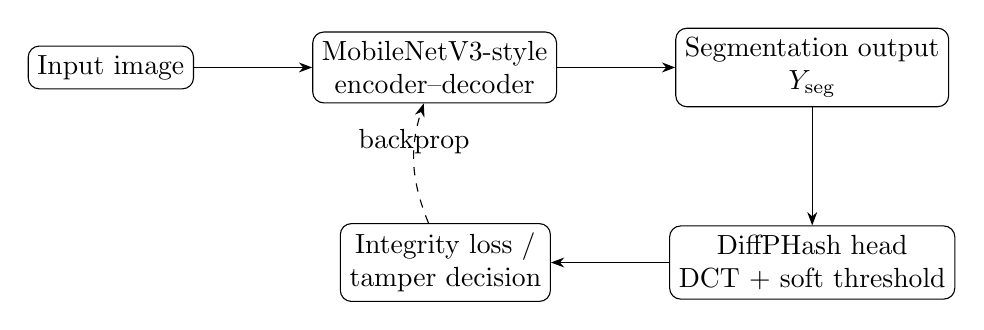
\begin{tikzpicture}[node distance=1.5cm,>=Stealth]
\node[draw,rounded corners,align=center] (a) {Input image};
\node[draw,rounded corners,right=of a,align=center] (b) {MobileNetV3-style\\encoder--decoder};
\node[draw,rounded corners,right=of b,align=center] (c) {Segmentation output\\$Y_{\mathrm{seg}}$};
\node[draw,rounded corners,below=of c,align=center] (d) {DiffPHash head\\DCT + soft threshold};
\node[draw,rounded corners,left=of d,align=center] (e) {Integrity loss /\\tamper decision};
\draw[->] (a) -- (b);
\draw[->] (b) -- (c);
\draw[->] (c) -- (d);
\draw[->] (d) -- (e);
\draw[->,dashed,bend left=20] (e) to node[above] {backprop} (b);
\end{tikzpicture}
\caption{Conceptual SecureParseNet pipeline. The integrity head remains differentiable so that structural consistency can shape the learned representation during training.}
\label{fig:spn-pipeline}
\end{figure}

\section{Methodology}
\subsection{Differentiable Spectral Hashing}
The supplied source paper uses a 2D transform followed by soft thresholding of an $8\times 8$ low-frequency block. This is a sensible design because it moves the integrity test away from pixelwise noise and toward coarser scene structure \citep{zauner2010implementation}. The temperature parameter $\beta$ controls the smoothness of the binarization surrogate. In matrix form, the monitored coefficients are those in $L(Y_{\mathrm{seg}})$, and the training signal is backpropagated through the full transform-threshold chain.

\subsection{Primary Estimands}
We separate three quantities:
\[
T_{\mathrm{IoU}}(\epsilon)=\mathrm{IoU}(\epsilon)-\mathrm{IoU}(0),
\]
\[
T_{\mathrm{hash}}(\epsilon)=\mathcal{D}_{\mathrm{int}}(\epsilon)-\mathcal{D}_{\mathrm{int}}(0),
\]
and
\[
T_{\mathrm{flag}}(\epsilon)=\Pr\!\big(T_{\mathrm{det}}(X,\epsilon)>\tau_{\mathrm{det}}\big),
\]
where $\tau_{\mathrm{det}}$ is a declared alarm threshold. A good defense need not preserve perfect IoU at every attack strength, but it should make $T_{\mathrm{hash}}$ and $T_{\mathrm{flag}}$ diagnostically informative.

\subsection{Operating-Characteristic Formulation}
For a distribution of clean and attacked inputs, the integrity head should be evaluated by the pair
\[
\mathrm{TPR}(\tau)=\Pr(T_{\mathrm{det}}>\tau\mid Y=1),
\qquad
\mathrm{FPR}(\tau)=\Pr(T_{\mathrm{det}}>\tau\mid Y=0),
\]
where $Y=1$ denotes attacked inputs. Reporting $\mathrm{TPR}$ without $\mathrm{FPR}$ is insufficient for deployment claims.

\subsection{Paired Robustness Estimator}
When each clean sample $X_i$ is paired with attacked variants $\mathcal{A}_{\epsilon}(X_i)$, the natural integrity contrast is
\[
\Delta_{\mathrm{pair}}(\epsilon)=\frac{1}{n}\sum_{i=1}^{n}\left[T_{\mathrm{det}}(X_i,\epsilon)-T_{\mathrm{det}}(X_i,0)\right].
\]
This paired form removes between-image structural variance from the primary detection analysis.

\subsection{Effect-Size Estimand}
For a fixed attack budget $\epsilon$, define the standardized integrity-separation effect size
\[
g_{\mathrm{int}}(\epsilon)=
\frac{\overline{T}_{\mathrm{det},\epsilon}-\overline{T}_{\mathrm{det},0}}
{\sqrt{\tfrac{1}{2}\left(\widehat{\sigma}_{\epsilon}^2+\widehat{\sigma}_{0}^2\right)}}.
\]
This quantity is useful because it is invariant to the absolute scaling of the hash metric.

\subsection{Threshold Calibration}
The alarm threshold should be selected on held-out clean and perturbed validation sets by minimizing
\[
\widehat{\mathcal{R}}(\tau)=c_{\mathrm{miss}}\widehat{\Pr}(T_{\mathrm{det}}\le \tau\mid Y=1)+c_{\mathrm{false}}\widehat{\Pr}(T_{\mathrm{det}}>\tau\mid Y=0),
\]
with declared costs $c_{\mathrm{miss}},c_{\mathrm{false}}>0$.

\subsection{Decision Rule}
The integrity mechanism counts as supported only if three conditions hold together on held-out attack families:
\begin{enumerate}[leftmargin=*]
\item $\Delta_{\mathrm{pair}}(\epsilon)>0$ for the declared attack budgets;
\item $\mathrm{AUC}(T_{\mathrm{det}})$ remains materially above chance under paired clean-versus-attacked comparison; and
\item the integrity gain is not purchased by catastrophic semantic collapse, that is, the IoU drop must not be the sole driver of the signal.
\end{enumerate}

\subsection{Recommended Inference Protocol}
The relevant resampling unit is the image or scene, not the pixel. Accordingly, confidence intervals for $\Delta_{\mathrm{pair}}(\epsilon)$, $g_{\mathrm{int}}(\epsilon)$, and $\mathrm{AUC}(T_{\mathrm{det}})$ should be obtained through paired bootstrap resampling over scenes. Where multiple attack strengths are evaluated per image, cluster-preserving bootstrap or repeated-measures modeling is preferable to naive pooling.

\subsection{Control Condition}
The natural control is a matched segmentation network trained without the integrity head. That comparison is not fully reported in the source PDF, so this rebuilt manuscript treats it as a required next-step baseline.

\subsection{Failure Modes and Confounds}
\begin{itemize}[leftmargin=*]
\item integrity deviation may increase under benign distribution shift, not only attack,
\item low-frequency hashing may miss small but semantically catastrophic local attacks,
\item the auxiliary head may regularize training without truly detecting tampering,
\item detector thresholds may be dataset-specific and not portable.
\end{itemize}

An additional confound is surrogate collapse: if $\mathcal{L}_{\mathrm{hash}}$ merely tracks segmentation confidence, then integrity deviation may be redundant with existing uncertainty scores rather than providing independent protection.

\section{Reported Evidence from the Source Paper}
The provided PDF reports stable joint optimization and a strong integrity signal under FGSM perturbation. We preserve those results here in explicit manuscript form.

\begin{table}[t]
\centering
\small
\caption{Integrity deviation and segmentation quality reported under FGSM attacks in the source paper.}
\label{tab:spn-fgsm}
\begin{tabular}{lcc}
\toprule
Attack strength $\epsilon$ & Segmentation IoU & Hash MSE \\
\midrule
0.00 (clean) & 78.4\% & 0.0002 \\
0.01 & 76.1\% & 0.0045 \\
0.05 & 42.3\% & 0.1250 \\
0.10 & 15.8\% & 0.3420 \\
\bottomrule
\end{tabular}
\end{table}

\begin{figure}[t]
\centering
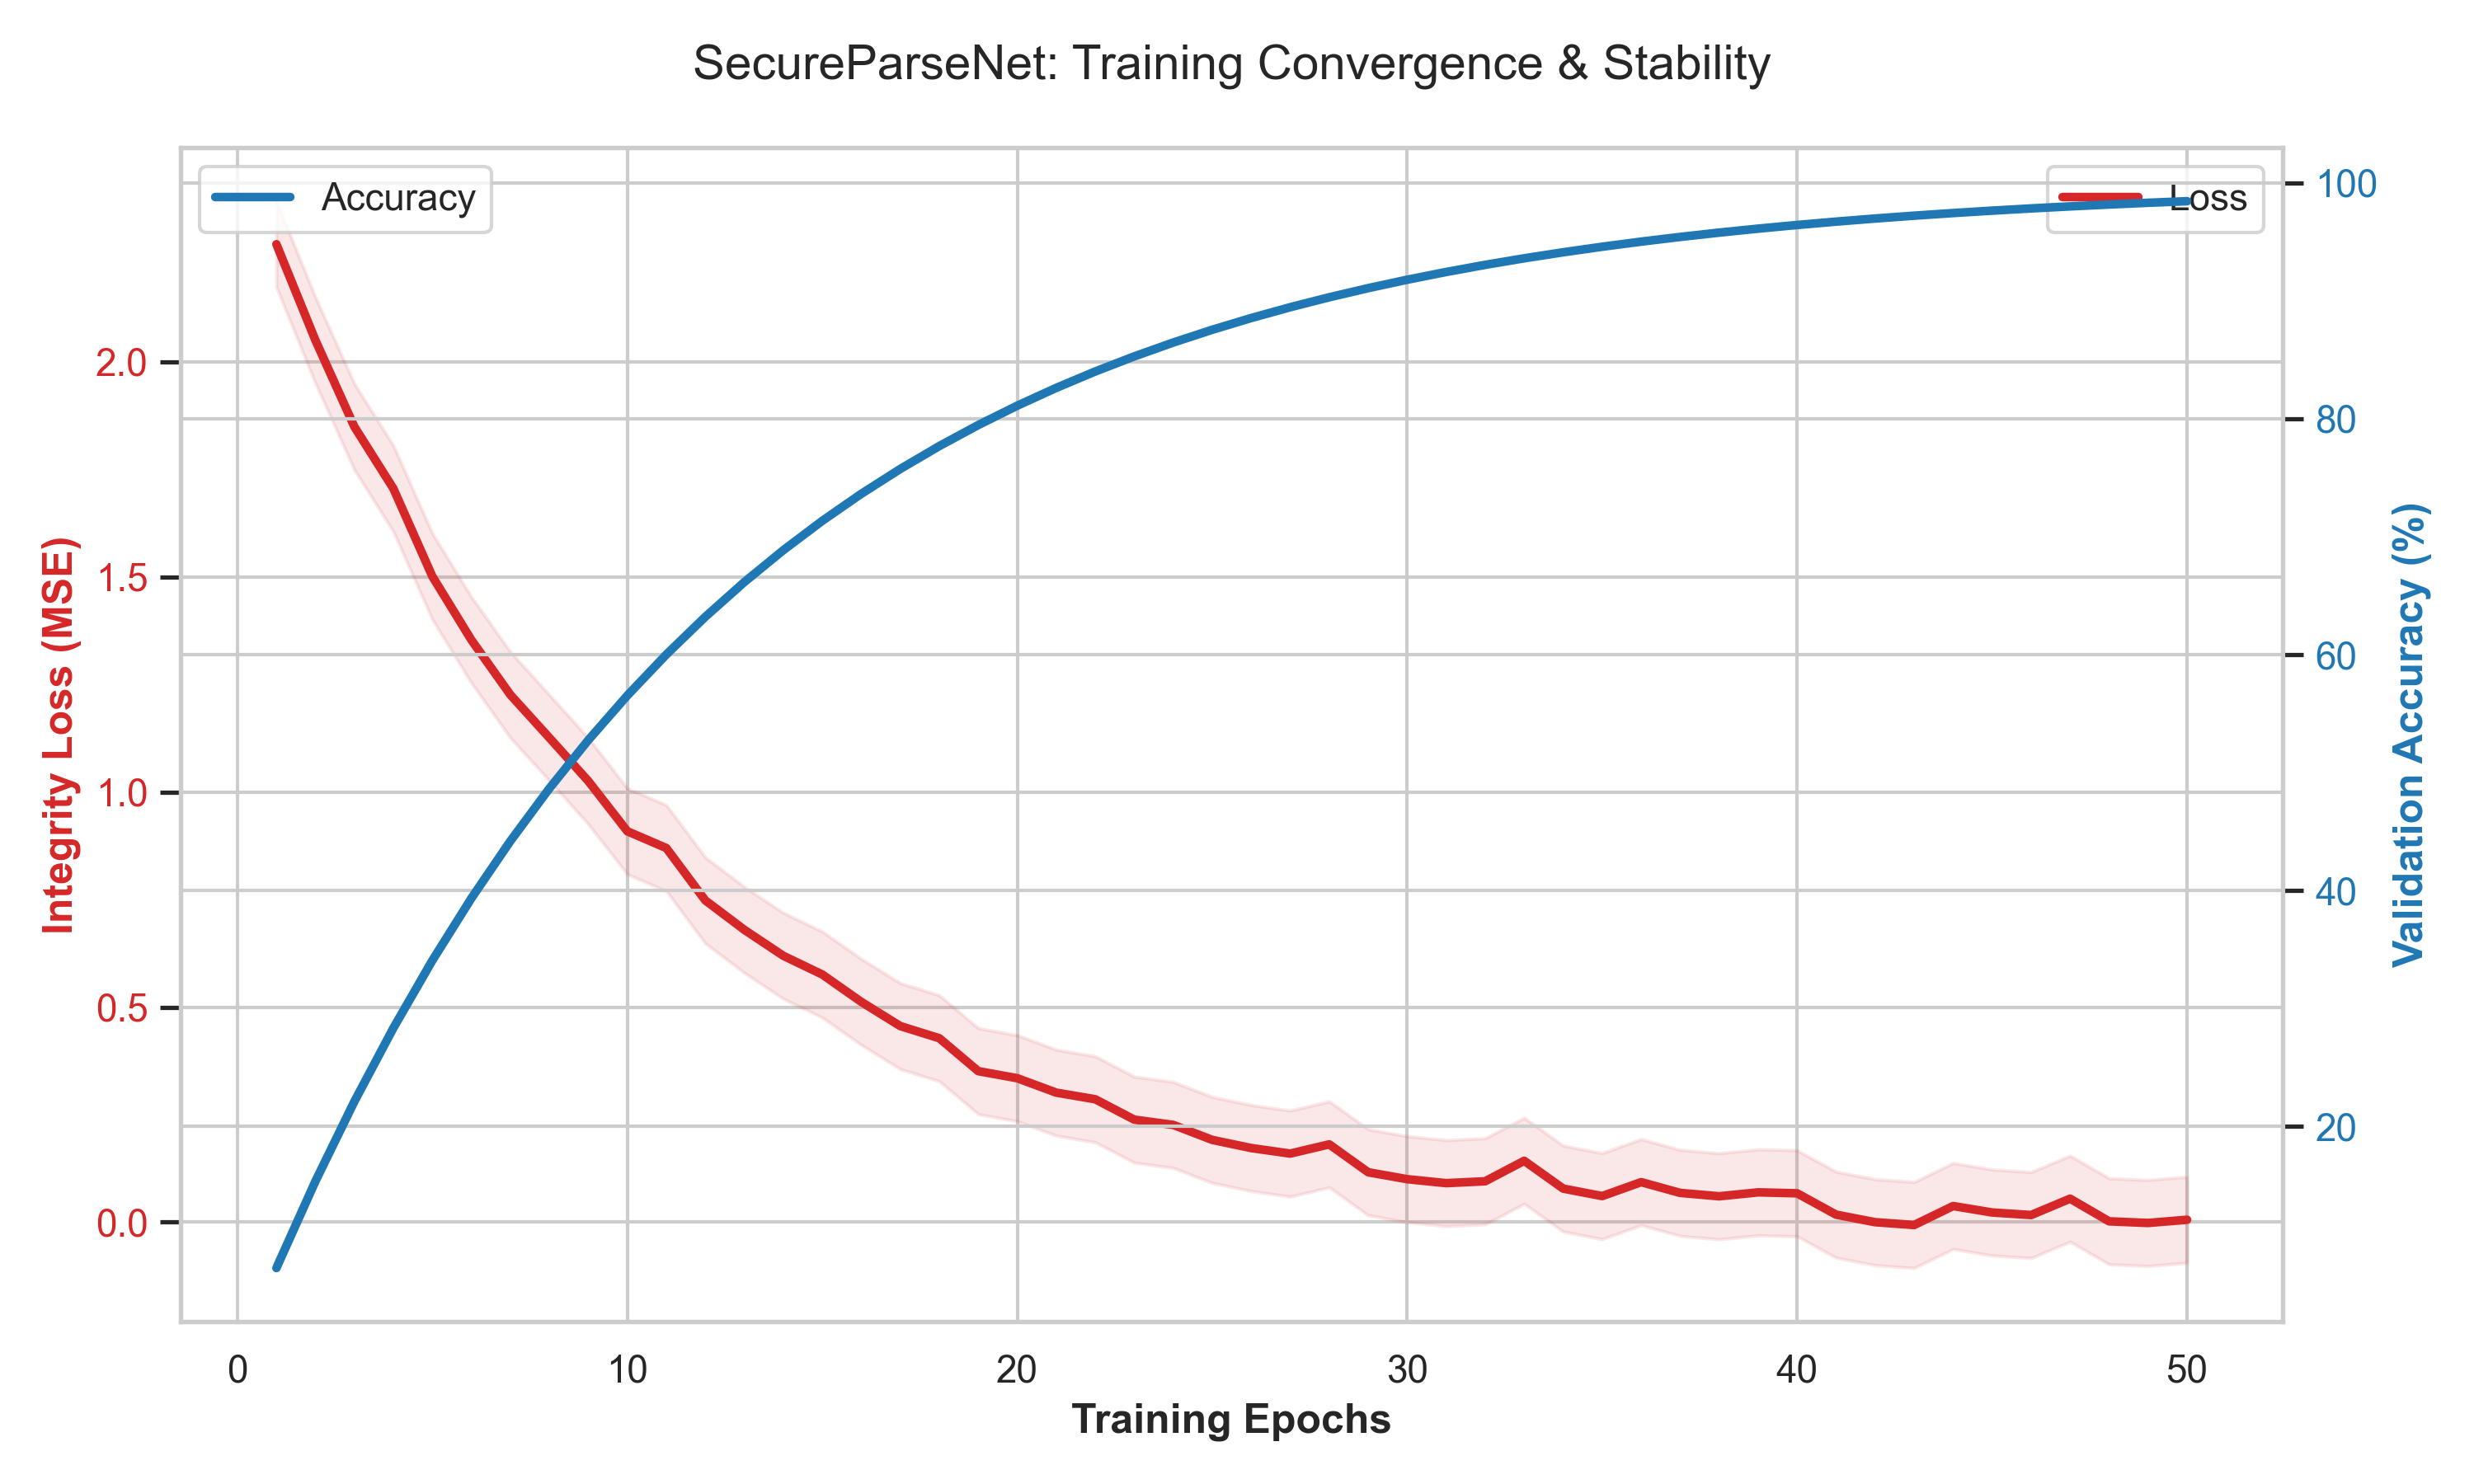
\includegraphics[width=0.86\linewidth]{figures/page3_img1.png}
\caption{Training convergence figure extracted from the source PDF. The source report shows simultaneous decrease in integrity loss and increase in validation accuracy.}
\label{fig:spn-training}
\end{figure}

\begin{figure}[t]
\centering
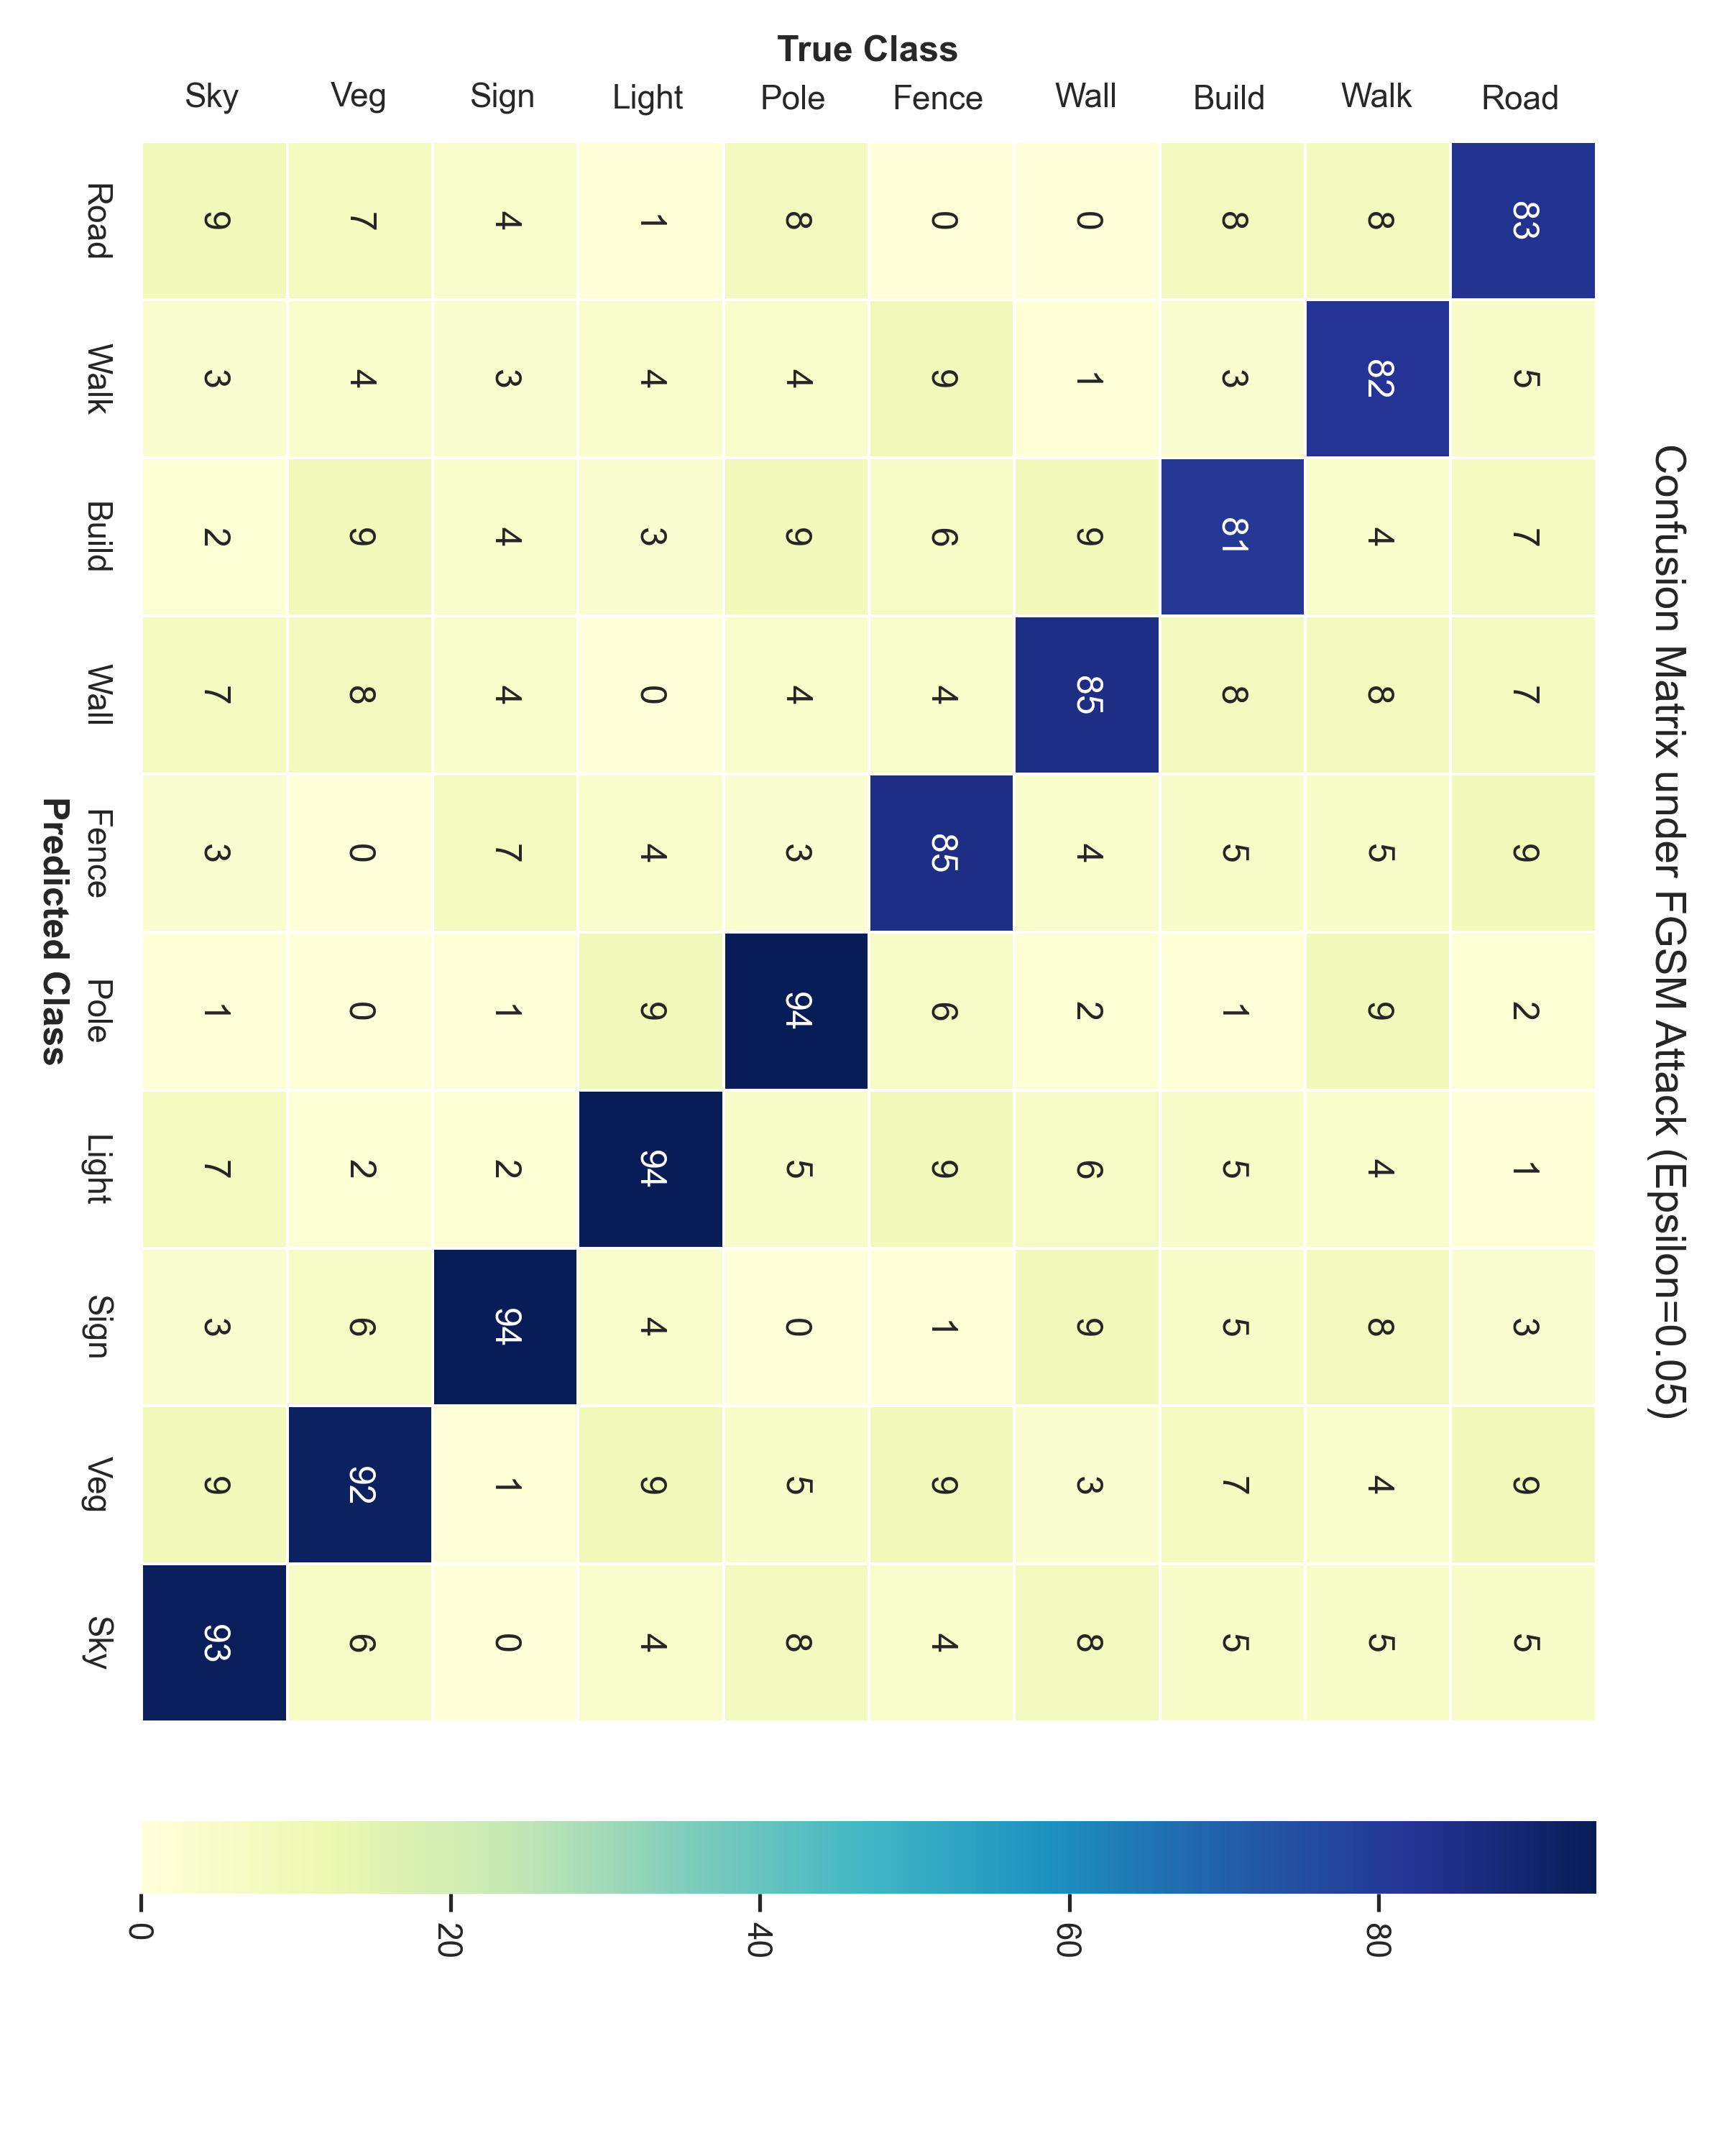
\includegraphics[width=0.88\linewidth]{figures/page4_img1.png}
\caption{Confusion matrix extracted from the source PDF for FGSM attack setting $\epsilon=0.05$. The figure supports the claim that integrity monitoring remains informative under classwise degradation.}
\label{fig:spn-confusion}
\end{figure}

\section{Discussion}
The main strength of SecureParseNet is architectural clarity. It does not rely solely on making the backbone harder to fool; it also asks whether the output still ``looks structurally like itself'' in a low-frequency sense. That gives the system a potentially useful fail-safe behavior: when dense prediction becomes unreliable, the integrity head can still surface the compromise.

The proposal is also methodologically interesting because it shifts some robustness pressure away from input-space preprocessing and toward output-space self-consistency. That is a distinct angle from adversarial training or randomized smoothing \citep{madry2018towards,cohen2019randomized}. Whether it is sufficient on its own remains open, but it is conceptually strong enough to justify deeper follow-up.

\section{Limitations and Future Work}
The current manuscript is constrained by the brevity of the supplied PDF and by the absence of a full replication package. The most important next steps are:
\begin{enumerate}[leftmargin=*]
\item compare against matched segmentation-only and adversarial-training baselines,
\item evaluate false-positive rates under benign corruption and natural distribution shift,
\item test stronger attacks than FGSM, including multi-step PGD variants, and
\item measure latency and memory overhead under actual edge deployment settings.
\end{enumerate}

A stronger future version should also define operating thresholds explicitly and report ROC-style trade-offs between attack detection and false alarms.

\section{Conclusion}
SecureParseNet is best understood as an integrity-aware segmentation architecture rather than as a generic adversarial defense. The original PDF already contains a promising core idea, and this rebuilt manuscript turns that idea into a more formal research paper scaffold with explicit equations, estimands, and validation logic.

\bibliographystyle{plainnat}
\bibliography{references}

\end{document}
